\chapter{Methodology}



\section{GIST}
% Outline Solution
The general idea of the presented solution combines three simple concepts:
\begin{itemize}
	\item The use of private characters as a unique key for a map. The value of the map is an object, thus a single character can be resolved to an arbitrary data structure.
	\item The parse tree is a tree data structure. If a part of the tree produced by a token sequence is saved in a single token, that token is a valid substitute for that part of the tree.
\end{itemize}
These two already allow to operate on the parse tree part in the map.
\begin{itemize}
	\item A parse tree constructor, which constructs a parse tree from an abstract syntax tree and is extensible, to assign types to and to skip parse tree construction for invisible elements. This allows the graphical editor to use the abstract syntax tree as data source directly. 
\end{itemize}

Figure \ref{ConceptFigure} shows the conceptional overview. 

On the right side of the diagram are the classical parser related elements, from below upwards:
\begin{itemize}
	\item a character stream
	\item a lexical analyzer or ``Lexer'', which reads the characters and groups them into Tokens.
	\item the token stream, which is produced by a Lexer and used by a Parser to create the ``Parse Tree''
\end{itemize}

On the left side is a ``Language Model'', which is deduced from the Parse Tree by the attribution of the grammar. In parser literature, \emph{this Language Model is called Abstract Syntax Tree}. The use of a modeling term instead of parsing term emphasizes where models are integrated and that a language description in modeling concepts is abstract. In contrast to context free grammars a language in modeling terms lacks a concrete notation. That the language model is equal to the abstract syntax tree is not mandatory. Until both data structured are combined in \ref{sec:MM:CFGs}, both terms are used. \\
The inverse transformation, from Language Model to Parse Tree is done by the Parse Tree Constructor. This transformation is ambiguous, because for one Language Model more than one valid Parse Tree can be constructed. \\
This described architecture is implemented in XText. This thesis conceptually extends the architecture by extending the Parse Tree Constructor, by the introduction of a ``Notation Model'' and an ``EMF Lexer''.
The Parse Tree Constructor is extended by 
\begin{itemize}
	\item adding valid alternative constructions to the Notation Model and regarding them while constructing the Parse Tree. 
	\item extensible rule evaluation capability to further specialize production parts depending on constraints.
	\item omitting Parse Tree branch construction for decorated Notation Model elements.
\end{itemize}
The Notation Model is introduced to:
\begin{itemize}
	\item be a serializable model
	\item to add an approved design of graphical editors to separating language elements and their corresponding notation state.
	\item to guide the Parse Tree constructor to be able to unambiguously construct a certain Parse Tree. This lead to a model with nearly the same expressive power as the Parse Tree itself, so the Notation Model was slightly extended to \emph{substitute the Parse Tree}. Figure \ref{ConceptFigure} shows the Notation Model separated from the Parse Tree as a bridge between Language Model and Parse Tree because this integration feature is the advantage of the Notation Model over the Parse Tree. The degree of overlapping functionality does not justify separated data structures.
\end{itemize} 
The EMF Lexer is introduced to:
\begin{itemize}
	\item separate private use characters from the character stream used for the original Lexer
	\item resolve the data structure identified by a private use character.
	\item determine a token name by properties of the \code{EObject}s in that data structure. This assignment process can be customized by additional rules that traverse the resolved data structure.
\end{itemize}


\begin{figure}
\centering
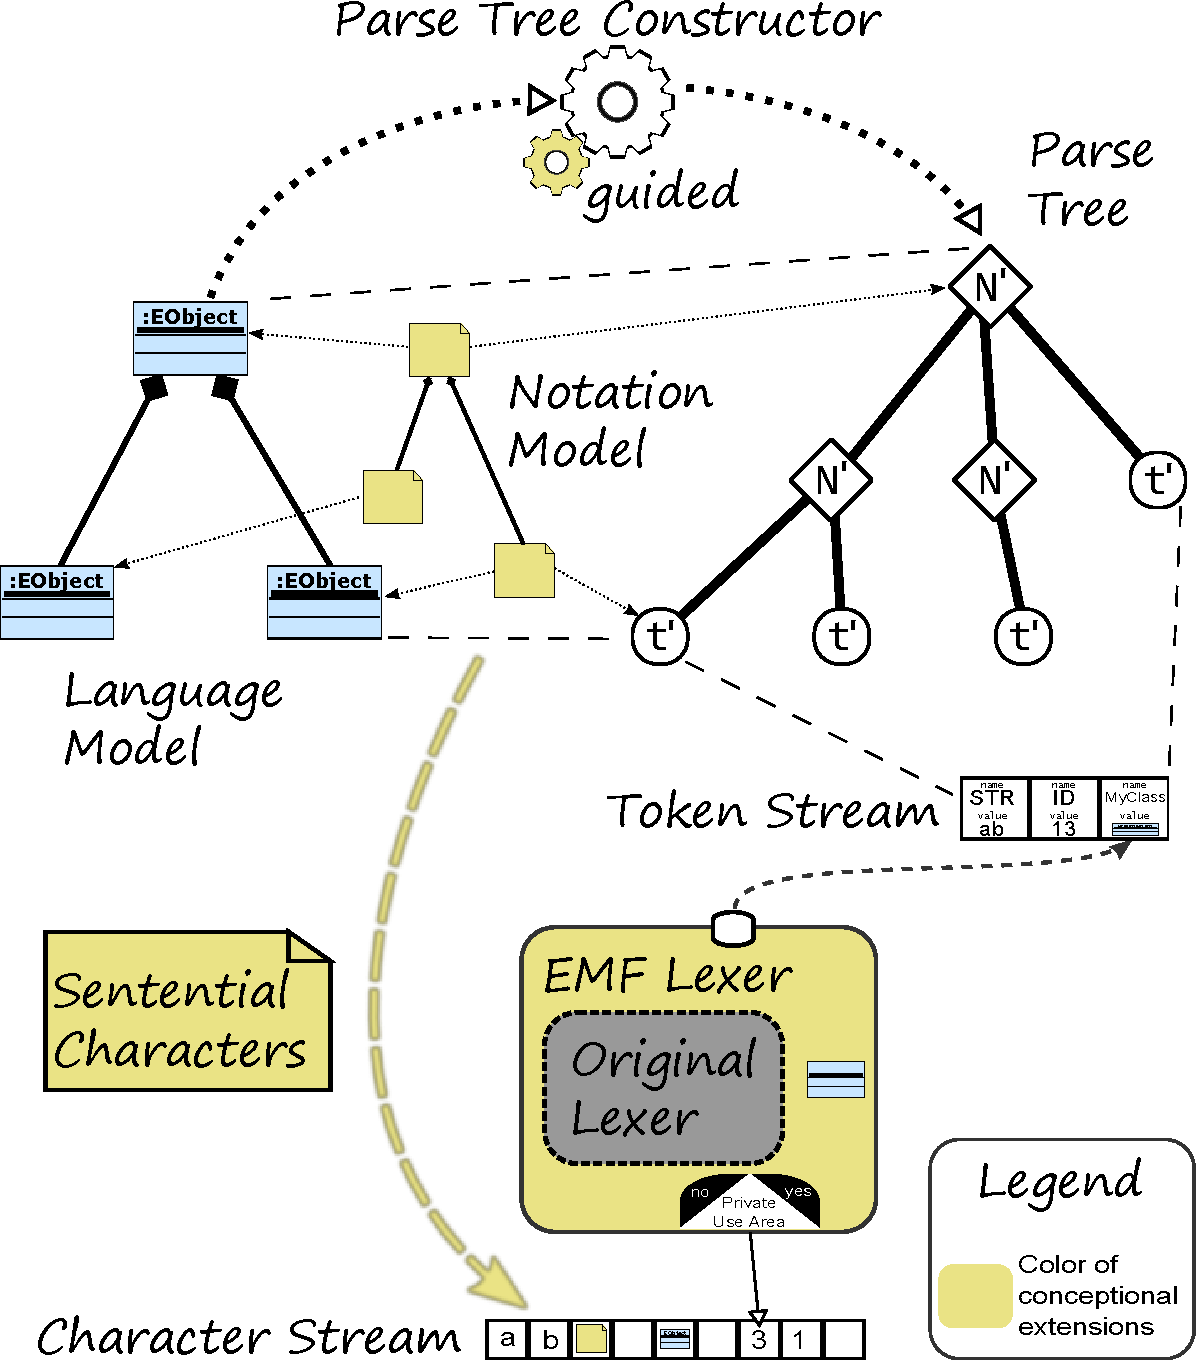
\includegraphics[scale=0.75]{gfx/ex/Concept} 
\caption{Conceptual Overview}
\label{ConceptFigure}
\end{figure}
